\subsection{Nguyên lý D'Alembert về công ảo}

\begin{frame}{Nguyên lý D'Alembert về công ảo}
\vspace{-4mm}
\begin{columns}
\column{0.4\textwidth}
    \begin{itemize}
        \item Nguyên lý công ảo
    \end{itemize}
    \begin{equation}
        \sum_{i} \left( \mathbf{F}_i - \dot{\mathbf{p}}_i \right) \cdot \delta \mathbf{r}_i = 0.
    \end{equation}
    \begin{itemize}
        \item Biến đổi sang tọa độ suy rộng
    \end{itemize}
    \begin{equation}
        \delta \mathbf{r}_i = \sum_{j} \frac{\partial \mathbf{r}_i}{\partial q_j} \delta q_j.
    \end{equation}


    \begin{itemize}
        \item Lực suy rộng
    \end{itemize}
    \begin{equation}
        Q_j = \sum_{i} \mathbf{F}^A_i \cdot \frac{\partial \mathbf{r}_i}{\partial q_j}.
    \end{equation}
    

\column{0.6\textwidth}
    \begin{itemize}
        \item Động lượng
    \end{itemize}
    \begin{equation}
        \dot{\mathbf{p}}_i = \frac{\mathrm{d}}{\mathrm{d} t} \left( \frac{\partial T}{\partial \dot{\mathbf{r}}_i} \right) = \left[ \frac{\mathrm{d}}{\mathrm{d} t} \left( \frac{\partial T}{\partial \dot{q}_j} \right) - \frac{\partial T}{\partial q_j} \right] \frac{\partial \mathbf{r}_i}{\partial q_j}.
    \end{equation}

    \begin{itemize}
        \item Nguyên lý D'Alembert
    \end{itemize}
    \begin{equation}
        \sum_{j} \left[ Q_j - \frac{\mathrm{d}}{\mathrm{d} t} \left( \frac{\partial T}{\partial \dot{q}_j} \right) + \frac{\partial T}{\partial q_j} \right] \delta q_j = 0.
    \end{equation}
    Ta thu được phương trình Euler-Lagrange
    \begin{equation}
        Q_j = \frac{\mathrm{d}}{\mathrm{d} t} \left( \frac{\partial T}{\partial \dot{q}_j} \right) - \frac{\partial T}{\partial q_j}.
    \end{equation}
\end{columns}
\end{frame}

\subsection{Tính toán lực bị động dựa trên phương trình Euler Lagrange}

\begin{frame}{Tính toán lực bị động dựa trên phương trình Euler Lagrange}
\vspace{-4mm}
\begin{itemize}
    \item Tăng thêm tọa độ suy rộng cho cơ hệ thay thế cho liên kết động học? \cite{morin2008introduction}
\end{itemize}
\begin{columns}
\column{0.5\textwidth}
    Lagrangian:
    \begin{equation}
        L = \frac{1}{2} m \left( \dot{r}^2 + \dot{\theta}^2 r^2 \right) -mg r \cos \left( \theta \right).
    \end{equation}

    Phương trình Euler-Lagrange
    \begin{equation}
        N = \frac{\mathrm{d}}{\mathrm{d} t} \left( \frac{\partial L}{\partial \dot{r}} \right) - \frac{\partial L}{\partial r} = m \ddot{r} - m \dot{\theta}^2 r + mg \cos \left( \theta \right).
    \end{equation}

    Tại \(r=R\) không đổi
    \begin{equation}
        N = -m \dot{\theta}^2 R + mg \cos \left( \theta \right).
    \end{equation}
    
\column{0.5\textwidth}
    \begin{figure}
        \centering
        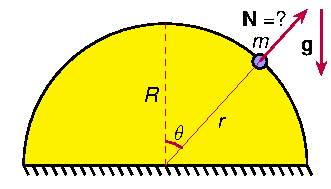
\includegraphics[width=0.9\linewidth]{Figures/Passive_force.pdf}
        \caption{Lực liên kết bị động \(\mathbf{N}\) được tính nhờ khảo sát tọa độ suy rộng \(r\).}
        \label{fig:Passive_force}
    \end{figure}

\end{columns}
\end{frame}

\subsection{Động lượng suy rộng và định lý Noether}

\begin{frame}{Động lượng suy rộng và định lý Noether}
\vspace{-4mm}
\begin{columns}
\column{0.5\textwidth}
    \begin{itemize}
        \item Lagrangian:
    \end{itemize}
    \begin{equation}
        L = \frac{7}{2} m \dot{x}^2 + 3 m \dot{x} \dot{y} + 2 m \dot{y}^2 - mg (x-2y). 
    \end{equation}
    Với phép biến đổi: \(x \to x_0 + \epsilon, y \to y_0 + 2\epsilon\) thì thành phần thế năng \(-mg (x_0 - 2 y_0)\) không phụ thuộc vào \(\epsilon\), nên \(\partial L / \partial \epsilon = 0\)

    \begin{itemize}
        \item Động lượng suy rộng
    \end{itemize}
    \begin{equation}
    \begin{split}
        p_{\epsilon} &= \frac{\partial L}{\partial \dot{x}} \frac{\partial x}{\partial \epsilon} + \frac{\partial L}{\partial \dot{y}} \frac{\partial y}{\partial \epsilon} \\
        &= 17 m \dot{x} + 10 m \dot{y} = \text{const}.
    \end{split}
    \end{equation}

\column{0.5\textwidth}
    \begin{figure}
        \centering
        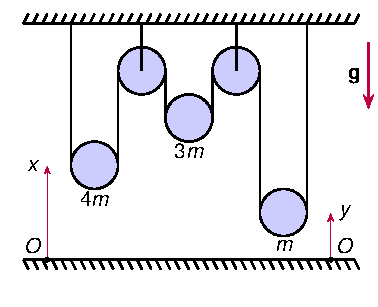
\includegraphics[width=0.9\linewidth]{Figures/Atwoods_machine.pdf}
        \caption{Hệ thống ròng rọc có động lượng suy rộng bảo toàn.}
        \label{fig:Atwoods_machine}
    \end{figure}
    
\end{columns}
\end{frame}

\begin{frame}{Cơ học Lagrange có phải lúc nào cũng là cách tiếp cận tốt nhất?}
\vspace{-2mm}
\begin{itemize}
    \item Lagrangian: \(L = \frac{1}{2} m_1 \dot{q}_1^2 + \frac{1}{2} m_2 \left[ \dot{q}_2^2 + \dot{q}_1^2 - 2 \dot{q}_1 \dot{q}_2 \cos (\theta) \right] - m_2 g q_2 \sin (\theta).\)
\end{itemize}

\begin{columns}
\column{0.5\textwidth}
    Phương trình Euler-Lagrange với \(q_1, q_2\)
    \begin{equation}
    \begin{split}
        & m_1 \ddot{q}_1 + m_2 \left[ \ddot{q}_1 - \ddot{q}_2 \cos (\theta) \right] = 0,\\
        & m_2 \left[ \ddot{q}_2 - \ddot{q}_1 \sin (\theta) \right] = - m_2 g \sin (\theta).
    \end{split}
    \end{equation}

    Hai phương trình trên có thể tìm được từ đâu?
    \begin{itemize}
        \item Bảo toàn động lượng phương nằm ngang.
        \item Định luật II Newton cho khối \(m_2\) chiếu theo phương song song mặt nghiêng.
    \end{itemize}

\column{0.5\textwidth}
    \begin{figure}
        \centering
        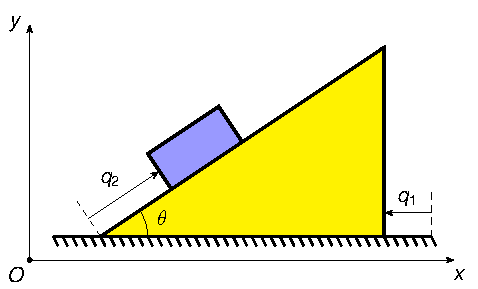
\includegraphics[width=0.9\linewidth]{Figures/Sliding_wedge.pdf}
        \caption{Nêm trượt trên nêm.}
        \label{fig:Sliding_wedge}
    \end{figure}
\end{columns}
\end{frame}

